\chapter{Pruebas del servicio web a trav'es de la aplicaci'on m'ovil} 
\label{capitulonueve}
Esta c'apitulo \ref{capitulonueve} se verifica las funciones de la etapa de prueba de servicio web este es una combinaci'on entre servicios. Es la etapa de verificar que nuestro servicio web brinde servicio a la aplicaci'on m'ovil. En el c'apitulo \ref{capituloseis} la aplicaci'on m'ovil realiza peticiones al servicio web y en el c'apitulo \ref{capitulocinco} el servicio web ofrece servicios de la p'agina del SAGAA. Uniendolos se empieza a validar el servicios web como se explica mas adelante.

\section{La etapa de prueba de descargar la planilla de notas con el servicio}
La etapa de prueba entre descargar la planilla de notas y el servicio se realiza en la funcionalidad de descargar la planilla de notas en los siguientes procesos: realizar la sesi'on del docente, listar la gesti'on, seleccionar la gesti'on, listar las carreras y selecci'onar la carrera para descargar la planilla de notas. A continuaci'on se muestra algunos de los servicios para descargar la planilla de notas.
\subsection{Prueba de sesi'on}
\label{Sesion}
La prueba de la sesi'on en el servicio se realiza en el 
desarrollo la sesi'on, al empezar la aplicaci'on m'ovil 'envian los datos al servicio el c'ual se encarga de enviar los par'ametros a la p'agina del SAGAA. Como se muestra en la figura \ref{fig:movilSesion} de la aplicaci'on m'ovil que 'envia los datos al servicio y en la figura \ref{fig:servicioSesion} es la ejecuci'on del servicio en el c'ual se muestra la conecci'on y la respuesta con la p'agina de SAGAA y obtiene la respuesta \textit{OK}. 
\begin{figure}[H]
\begin{minipage}{0.48\textwidth}
\centering
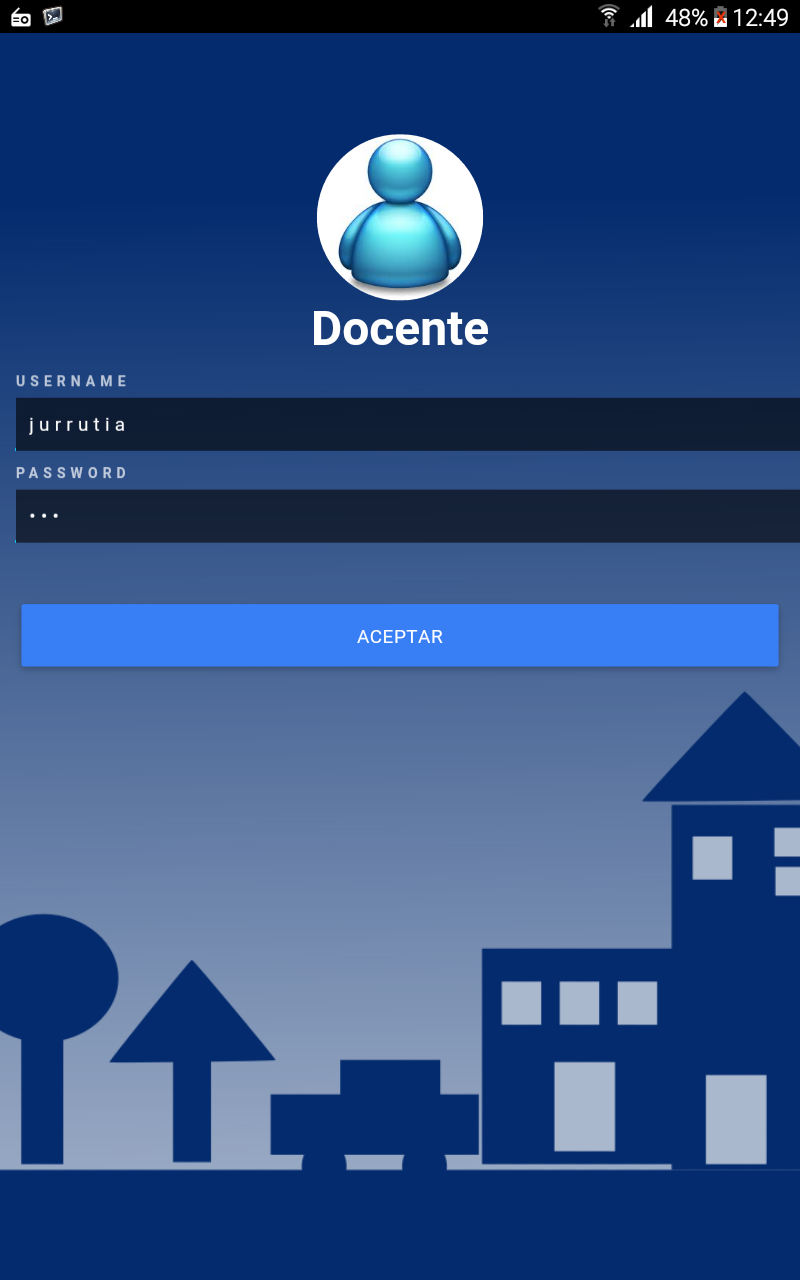
\includegraphics[width=.4\linewidth]{movilSesion.png}
\caption{La aplicaci'on m'ovil solicita la sesi'on al servicio web, Fuente: Elaboraci'on propia}
\label{fig:movilSesion}
\end{minipage}\hfill
\begin {minipage}{0.48\textwidth}
\centering
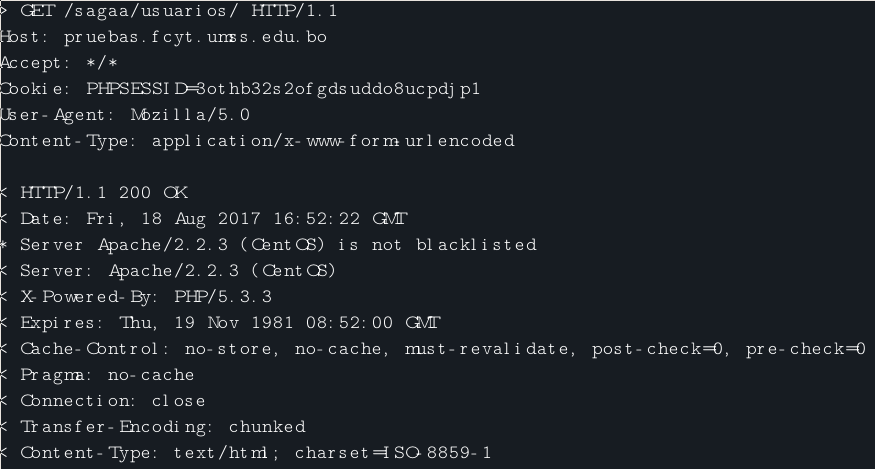
\includegraphics[width=.9\linewidth]{servicioSesion.png}
\caption{Respuesta de la p'agina del SAGAA al servicio web, Fuente: Elaboraci'on propia}
\label{fig:servicioSesion}
\end{minipage}
\end{figure}


%\subsection{Listar la gesti'on}

%\begin{figure}[H]
%   \begin{minipage}{0.48\textwidth}
%     \centering
%     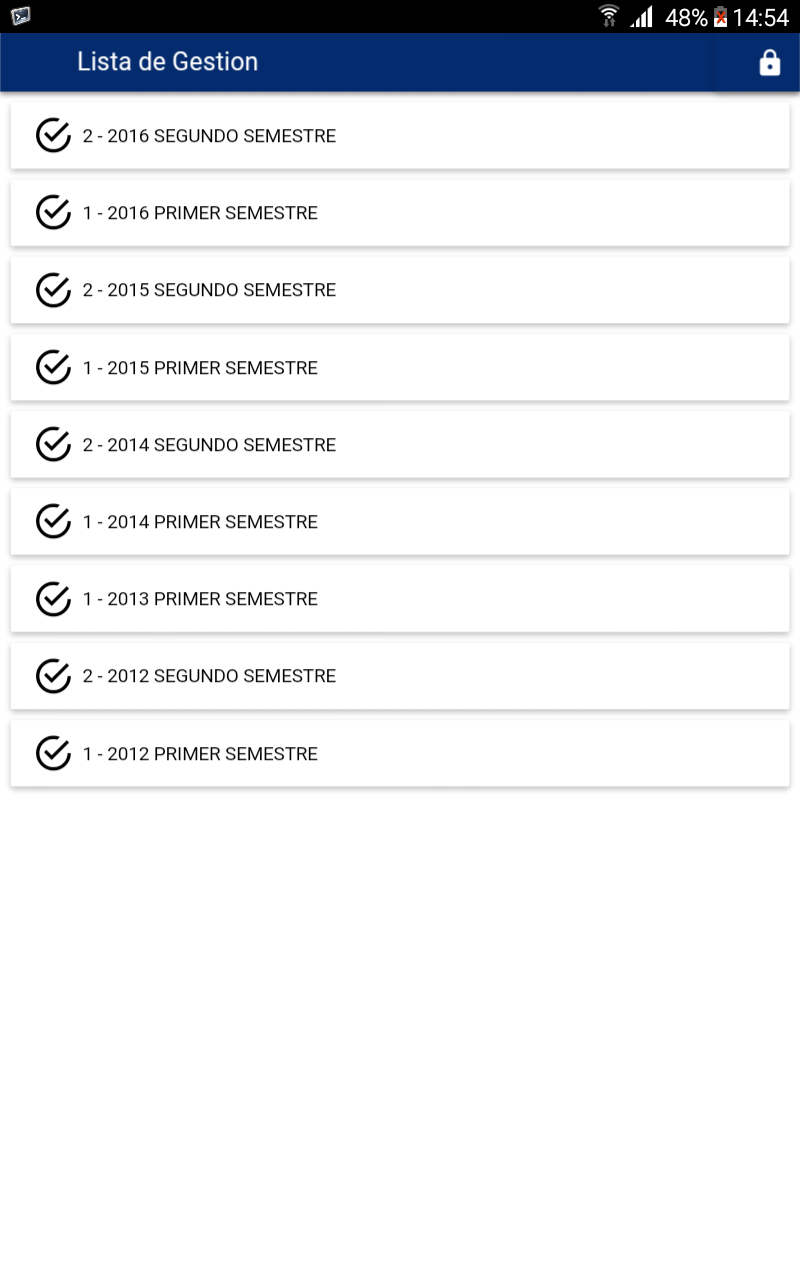
\includegraphics[width=.4\linewidth]{movilGestion.png}
%     \caption{Aplicaci'on m'ovil lista de gesti'on}\label{fig:movilGestion}
%   \end{minipage}\hfill
%   \begin {minipage}{0.48\textwidth}
%     \centering
%     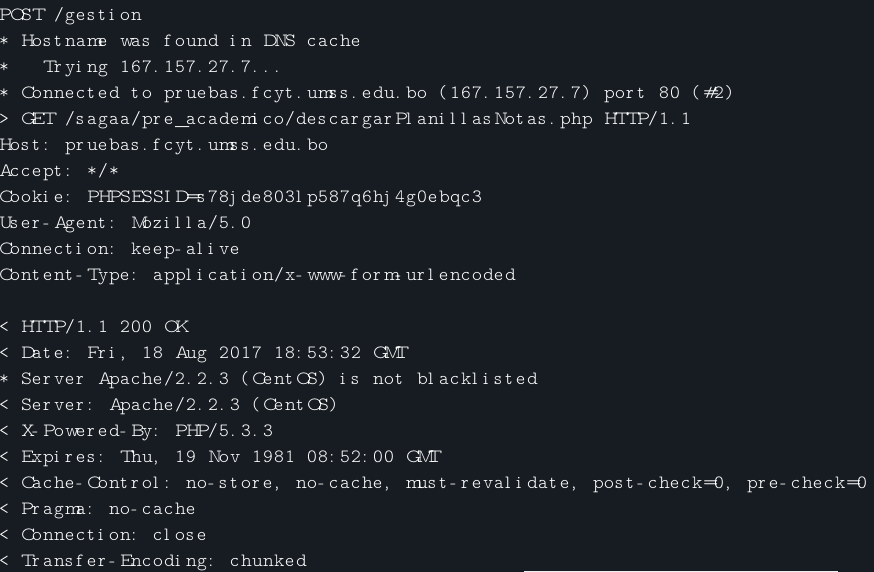
\includegraphics[width=.9\linewidth]{servicioGestion.png}
%     \caption{Respuesta de la lista de gesti'on}\label{fig:servicioGestion}
%   \end{minipage}
%\end{figure}

%\subsection{Seleccionar la gesti'on retorna la lista de carreras}
%\begin{figure}[H]
%   \begin{minipage}{0.48\textwidth}
%     \centering
%     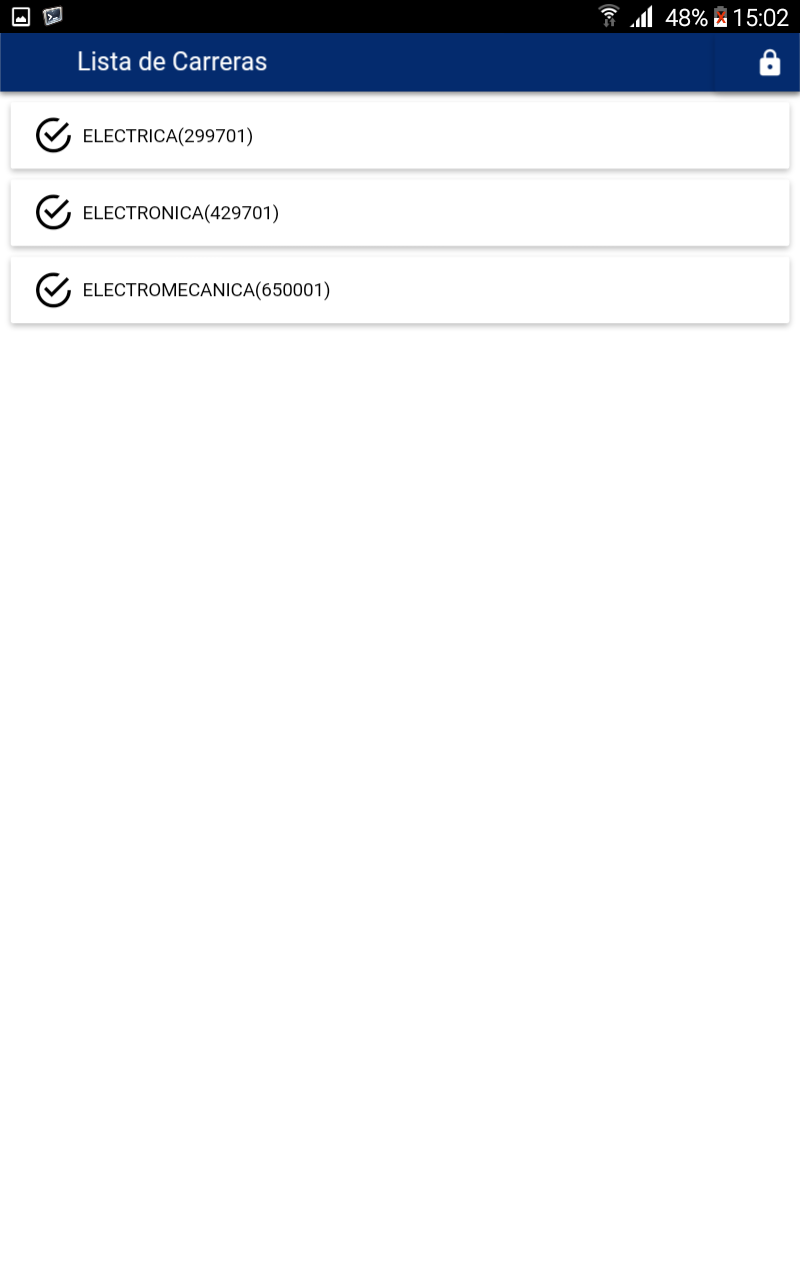
\includegraphics[width=.4\linewidth]{movilCarrera.png}
%     \caption{Aplicaci'on m'ovil seleccionar una gesti'on}\label{fig:movilSeleccionar}

%   \end{minipage}\hfill
%  \begin {minipage}{0.48\textwidth}
%     \centering
%     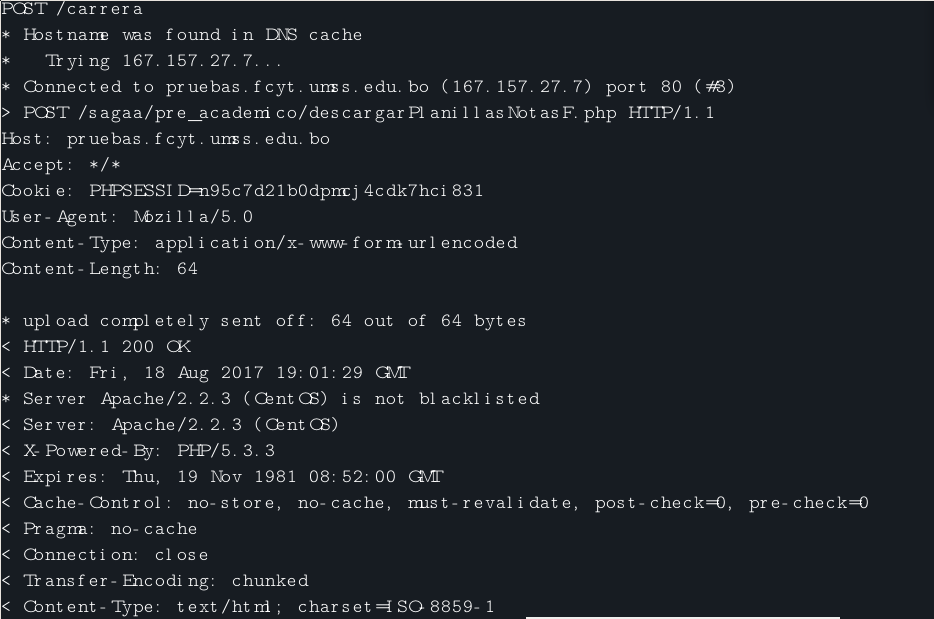
\includegraphics[width=.9\linewidth]{servicioCarrera.png}
%     \caption{Respuesta de seleccionar la lista de gesti'on}\label{fig:servicioSeleccionar}
%   \end{minipage}
%\end{figure}

\subsection{Prueba de descargar la planilla de notas}
La prueba de descargar la planilla de notas se realiza sobre la funcionalidad de descargar la planilla de notas, primeramente se han elegido la gesti'on, el detalle de la carrera y finalmente elige la opci'on  de descargar planilla de notas. La siguiente figura \ref{fig:movilDescargar} es la aplicaci'on m'ovil que solicita la descarga de la planilla de notas al servicio web, a tr'aves del icono descargar. En la figura \ref{fig:servicioDescargar}es la ejecuci'on del servicio web, el c'ual muestra una conecci'on y la respuesta con  p'agina del SAGAA y obtiene la planilla de notas. 

\begin{figure}[H]
\begin{minipage}{0.48\textwidth}
\centering
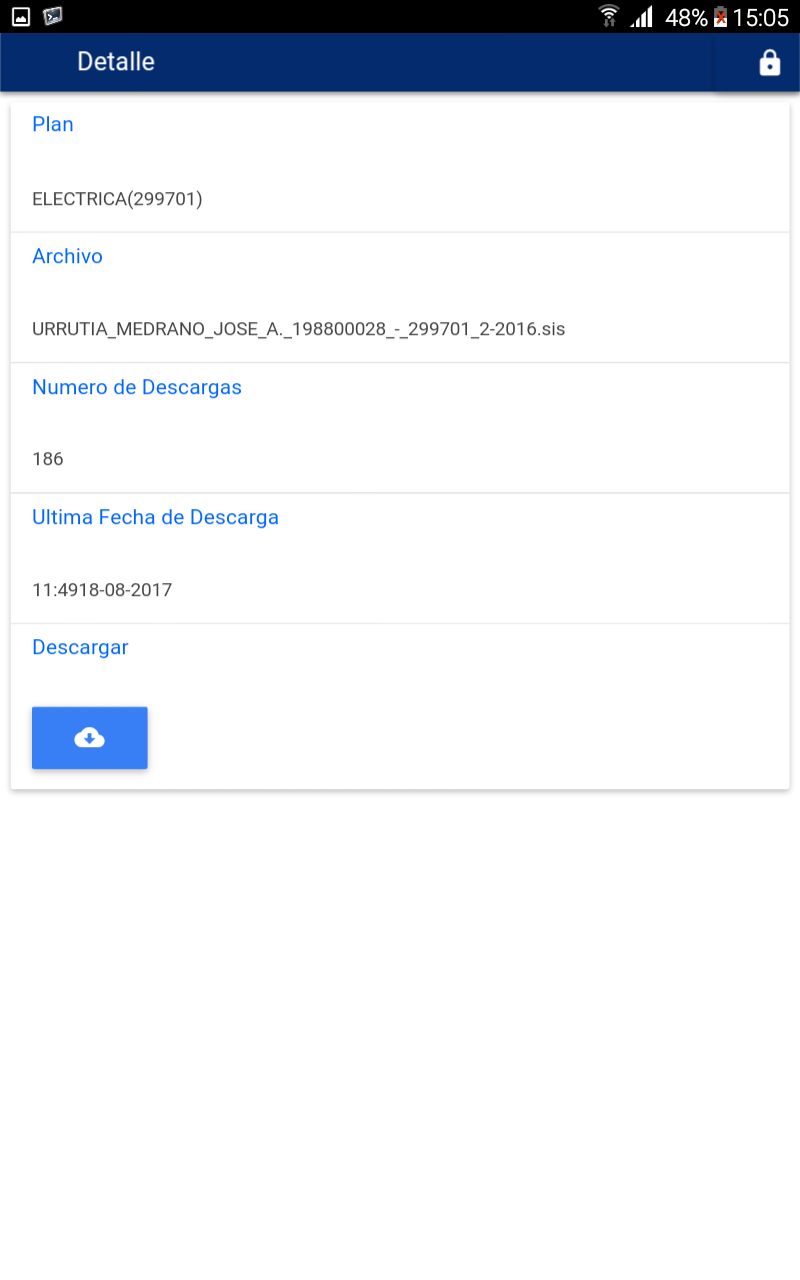
\includegraphics[width=.4\linewidth]{movilDescarga.png}
\caption{Seleccionar la carrera para descargar la planilla de notas, Fuente: Elaboraci'on propia}
\label{fig:movilDescargar}
\end{minipage}\hfill
\begin {minipage}{0.48\textwidth}
\centering
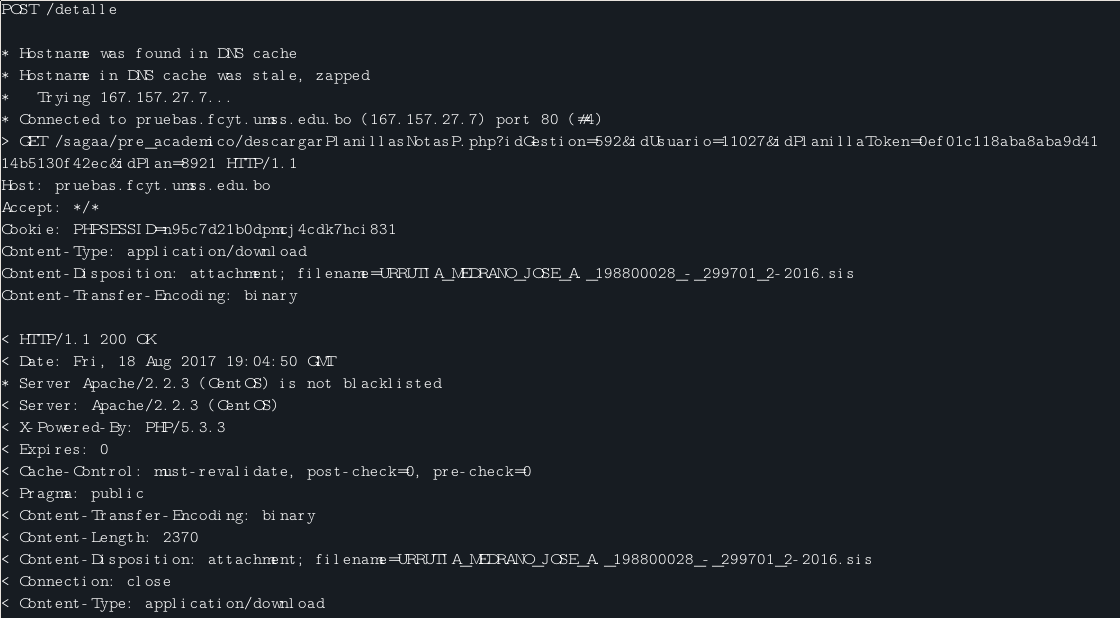
\includegraphics[width=.9\linewidth]{servicioDescarga.png}
\caption{Descargar la planilla de notas, Fuente: Elaboraci'on propia}
\label{fig:servicioDescargar}
\end{minipage}
\end{figure}

\section{La etapa de prueba de modificar la planilla de notas y el servicio}
En la etapa de prueba de modificar la planilla de notas se realizo a partir de la  prueba de la sesi'on como se muestra  en la seccion \ref{Sesion}. Despu'es se ha  guardado la planilla de notas en el servidor local del servicio y despu'es se filtran los datos y  convierten la planilla de notas en una unidad de datos json y se 'envia a la aplicaci'on m'ovil para mostrarlo. A  continuaci'on se muestra la validaci'on de algunos servicios: 

\subsection{Prueba de filtrar y convierte la planilla de notas}
La prueba de filtrar y convertir la planilla de notas, al comienzo se ha eliminado el inicio y fin para convertirlo a json. En las siguientes figuras \ref{fig:servicioFiltrar}, \ref{fig:crearJson} es la ejecuci'on del servicio.
\begin{figure}[H]
\begin{minipage}{0.48\textwidth}
\centering
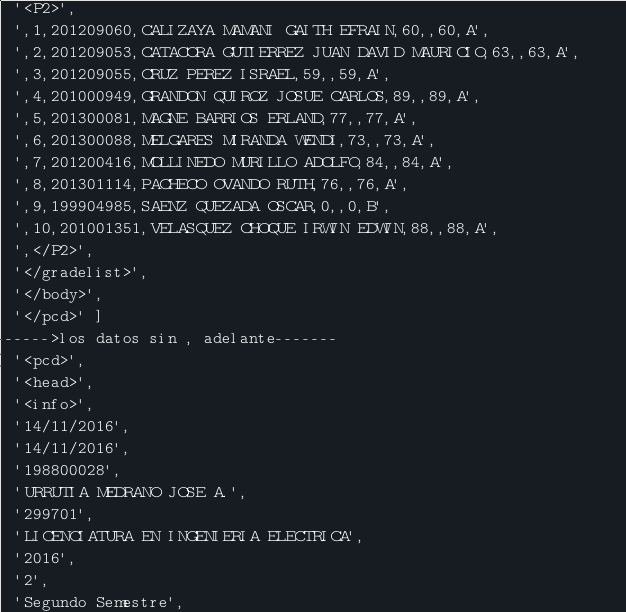
\includegraphics[width=.4\linewidth]{filtraPlanilla.png}
\caption{Lista los datos de la planilla de notas, Fuente: Elaboraci'on propia}
\label{fig:servicioFiltrar}
\end{minipage}\hfill
\begin {minipage}{0.48\textwidth}
\centering
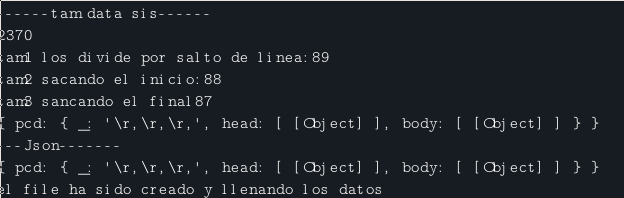
\includegraphics[width=.9\linewidth]{crearJson.png}
\caption{Envia los datos de la planilla de notas en Json, Fuente: Elaboraci'on propia}
\label{fig:crearJson}
\end{minipage}
\end{figure}

Despu'es de filtrar y convertir la planilla de notas se envia la unidad de datos json a la aplicaci'on movil para empezar a modificar.

\subsection{La prueba de reconocer la planilla de notas en la aplicaci'on m'ovil}
A partir de los puntos anteriores se comienza con la prueba de estrucutura  la planilla de notas. La aplicaci'on m'ovil solicita el archivo de planilla de notas. Esta aplicaci'on debe de reconocer y ordenar como se muestra en las siguientes figuras. 
\begin{figure}[H]
\begin{minipage}{0.33\textwidth}
\centering
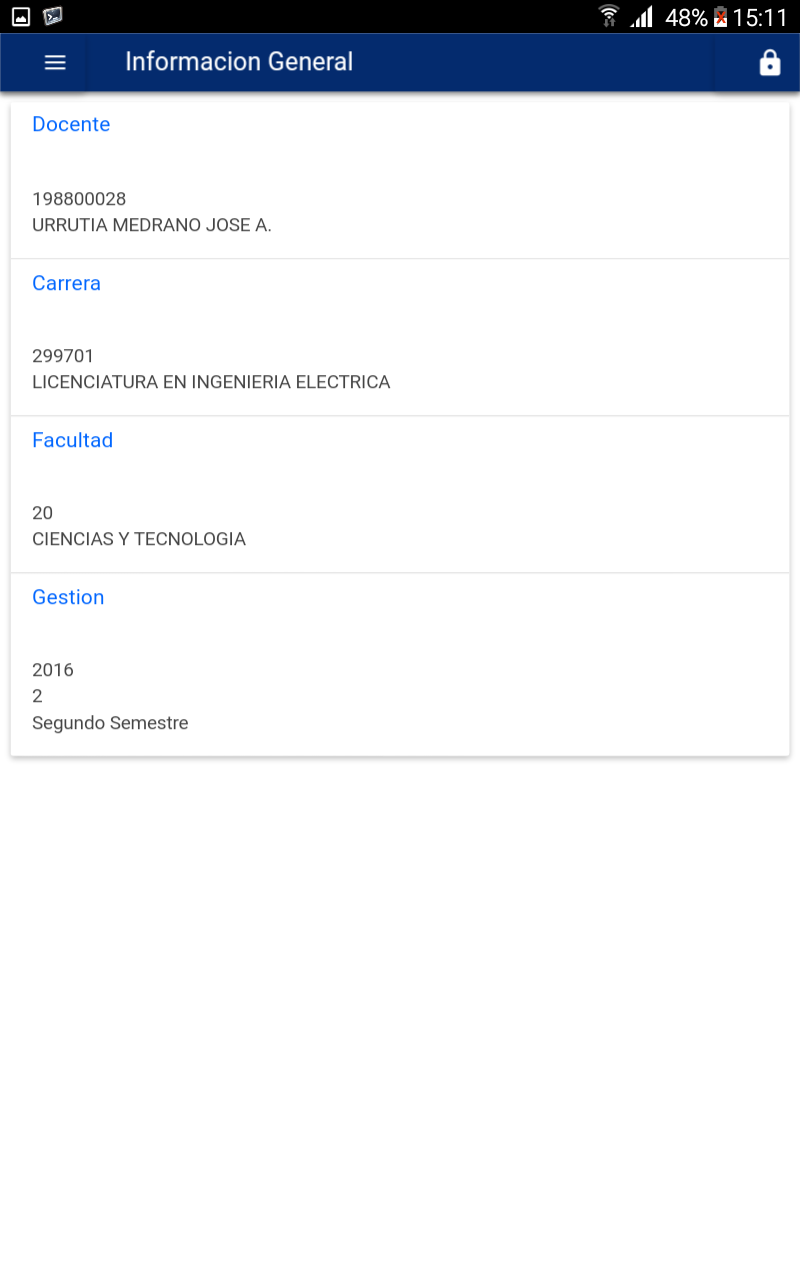
\includegraphics[width=0.4\linewidth]{movilMostrarJson.png}
\caption{Informaci'on general, Fuente: Elaboraci'on propia}
\label{fig:movilInfGral}
\end{minipage}\hfill
\begin{minipage}{0.33\textwidth}
\centering
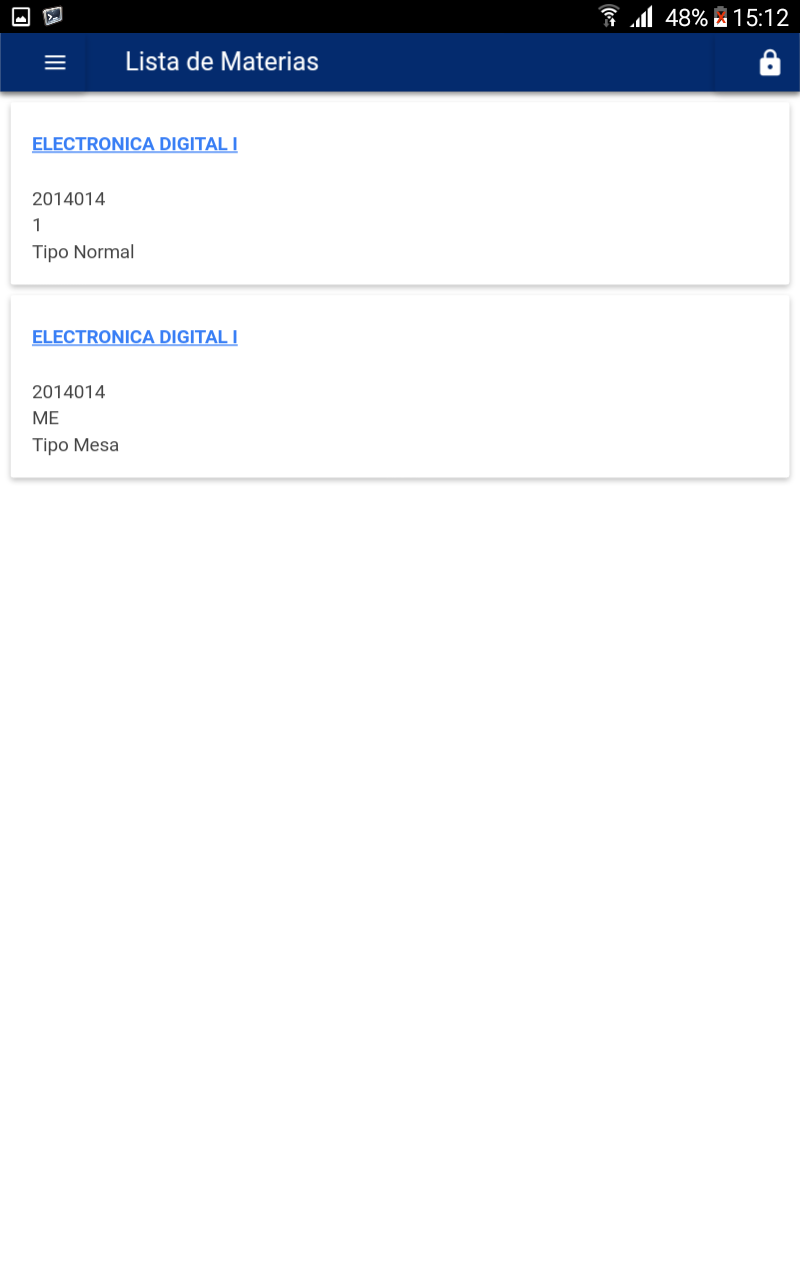
\includegraphics[width=0.4\linewidth]{movilMostrarJsonG.png}
\caption{La informaci'on de los grupos, Fuente: Elaboraci'on propia}
\label{fig:movilGrupo}
\end{minipage}\hfill
\begin{minipage}{0.33\textwidth}
\centering
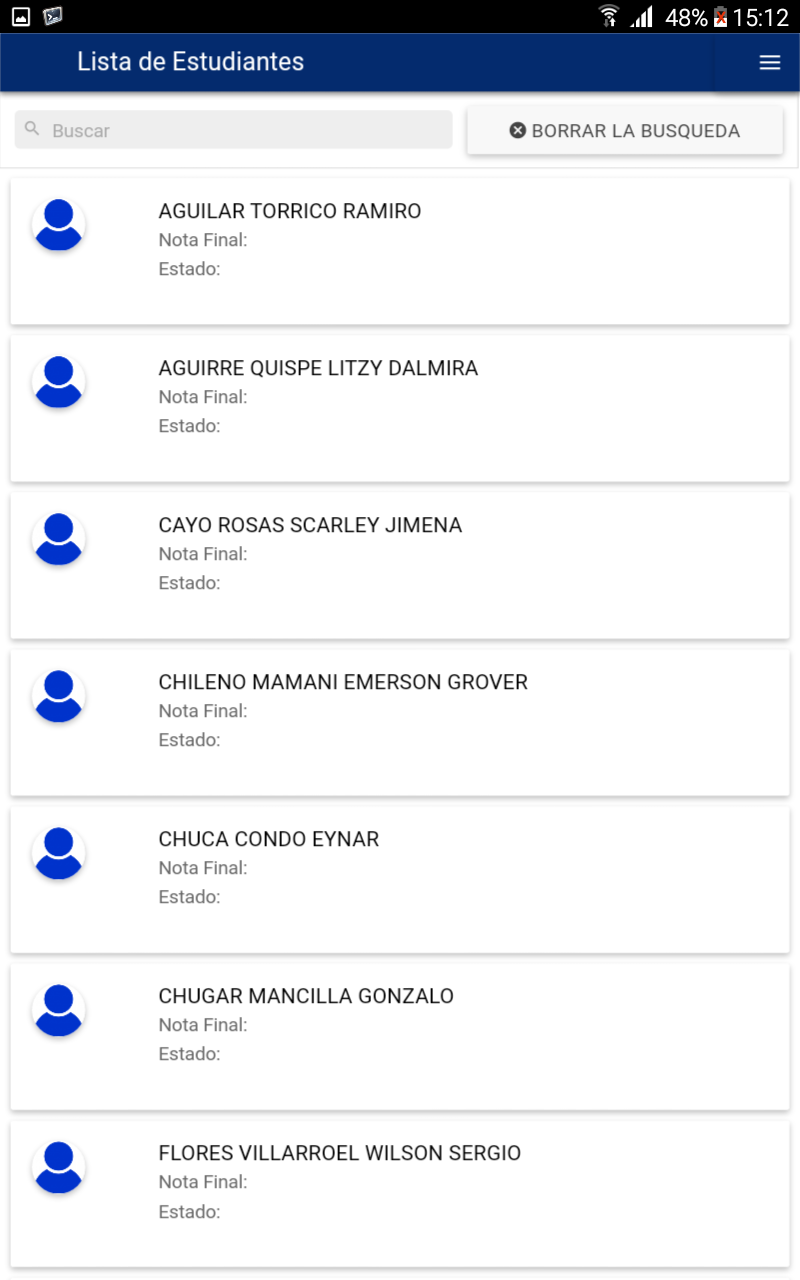
\includegraphics[width=.4\linewidth]{movilModificarJsonG.png}
\caption{La lista de estudiantes, Fuente: Elaboraci'on propia}
\label{fig:movilEstudiantes}
\end{minipage}
\end{figure}
La descripci'on de las figuras son: la figura \ref{fig:movilInfGral} muestra la informaci'on general, en la figura \ref{fig:movilGrupo} lista los grupos y en la figura \ref{fig:movilEstudiantes} muestra la lista de estudiantes.  

Despues de concluir con esta etapa de prueba realiza el proceso de guarda los datos modificados, este proceso 'envia la planilla de notas modificada al servicio.

\subsection{La prueba de modificar la planilla de notas en el servicio} 
La prueba de modificar la planilla de notas se trata de  armar la estrutura que reconoce la p'agina del SAGAA, tambi'en de buscar y reemplazar datos modificados. Por ultimo este archivo de planilla de notas modificados debe enviar a la p'agina del SAGAA como se observa en las siguientes figuras  \ref{fig:servicioGuardar}, \ref{fig:servicioModificar}.

\begin{figure}[H]
\begin{minipage}{0.48\textwidth}
\centering
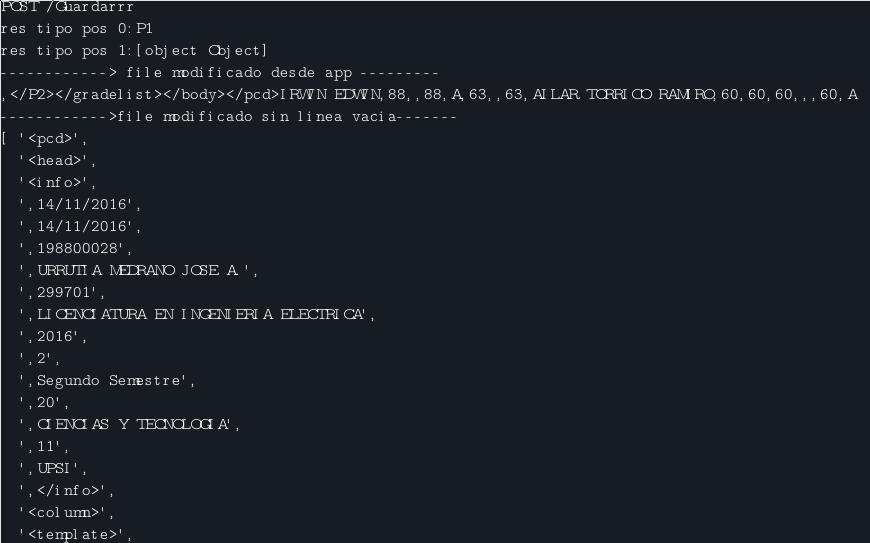
\includegraphics[width=.4\linewidth]{servicioGuardar.png}
\caption{El servicio web, recibe la planilla de notas, Fuente: Elaboraci'on propia}
\label{fig:servicioGuardar} 
\end{minipage}\hfill
\begin{minipage}{0.48\textwidth}
\centering
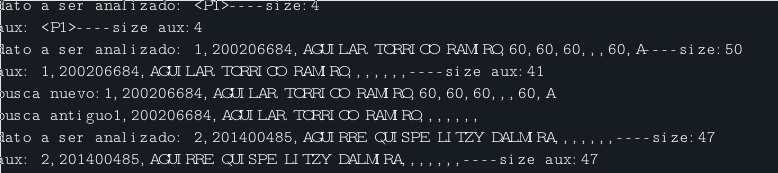
\includegraphics[width=.9\linewidth]{servicioModificar.png}
\caption{El servicio web, busca y reemplaza los datos modificado en la planilla de notas, Fuente: Elaboraci'on propia}
\label{fig:servicioModificar}
\end{minipage}
\end{figure}

\section{La etapa de prueba de adjuntar la planilla de notas} 
La etapa de prueba de adjuntar la planilla de notas se desarrolla las funcionalidades de: eligir la gesti'on, elegir el tipo de grupo y  adjuntar el archivo de planilla de notas.


En la siguiente figura \ref{fig:servicioAdjuntarG1} se muestra la petici'on y la respuesta de la selecci'on  de gesti'on y el adjuntar la planilla de notas y en la figura \ref{fig:servicioHabilitarG} es la petici'on y la respuesta de la selecci'on de grupo.   

\begin{figure}[H]
\begin{minipage}{0.48\textwidth}
\centering
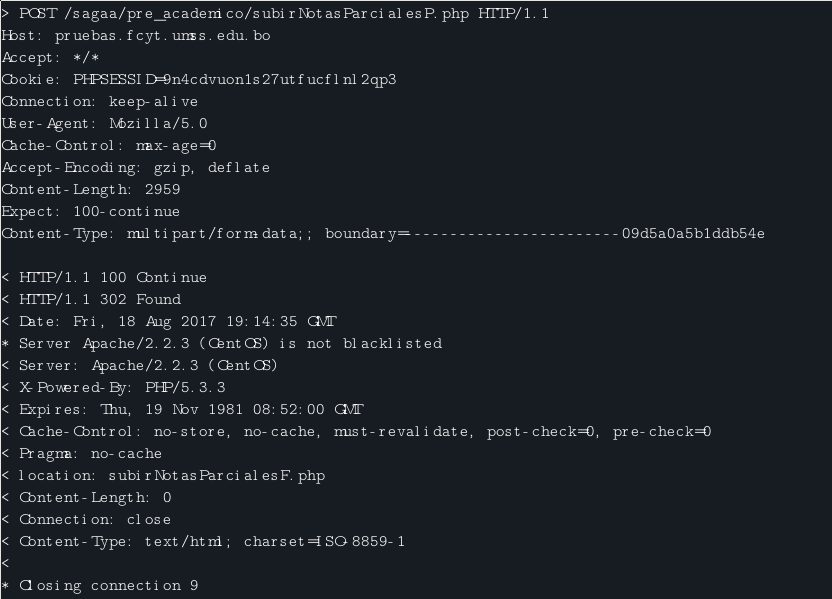
\includegraphics[width=.9\linewidth]{servicioAdjuntarG.png}
\caption{El servicio web, envia la gestion y adjunta la planilla de notas, Fuente: Elaboraci'on propia}
\label{fig:servicioAdjuntarG1}
\end{minipage}\hfill
\begin{minipage}{0.48\textwidth}
\centering
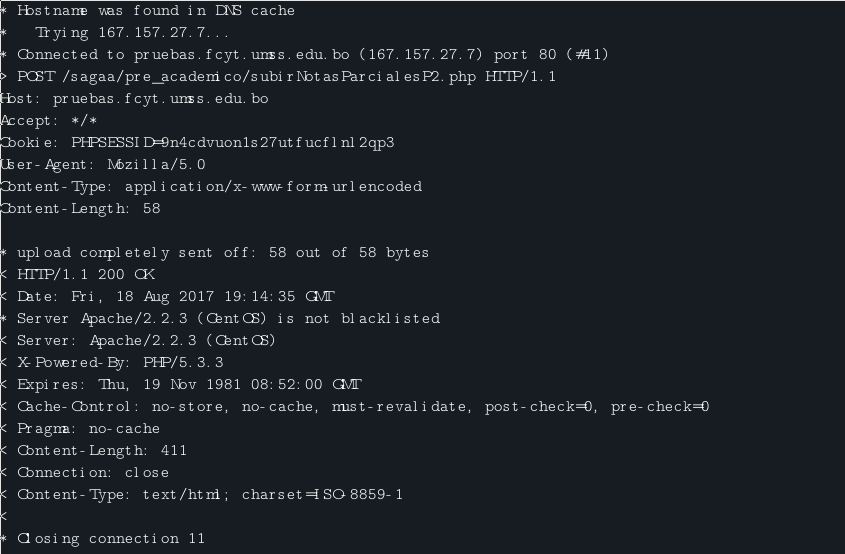
\includegraphics[width=.9\linewidth]{servicioHabilitarG.png}
\caption{El servicio web, 'envia el grupo que debe ser modificado, Fuente: Elaboraci'on propia}
\label{fig:servicioHabilitarG}
\end{minipage}
\end{figure}

%\subsection{Es la etapa de prueba de seleccionar el grupo para habilitar estudiante}
%Despu'es de adjuntar y seleccionar la gessti'on . Despu'es se 'envia a la p'agina del SAGAA, el c'ual  responde con un mensaje \textit{Finalizo la habilitaci'on de estudiantes y el cargado de planillas.}
\begin{figure}[H]
\centering
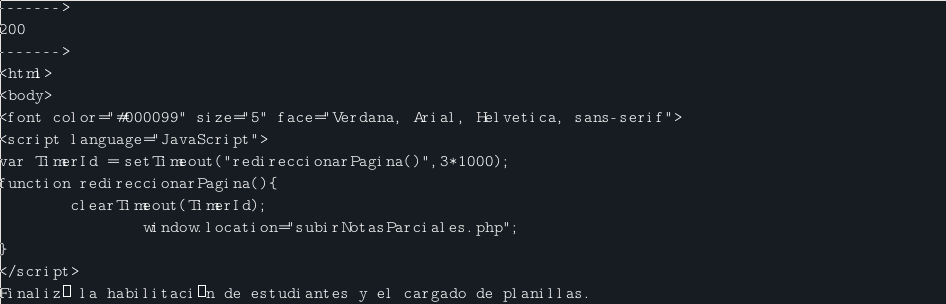
\includegraphics[width=0.8\textwidth]{servicioHabilitar.png}
\captionsetup{justification=centering, margin=2cm}
\caption{En el servicio web, es la respuesta de la p'agina del SAGAA, Fuente: Elaboraci'on propia}
\label{fig:habilitadoG}
\end{figure}
En la figura \ref{fig:habilitadoG} se muestra la respuesta de elegir el grupo de la planilla de notas.
